% experimental.tex
\documentclass[main.tex]{subfiles}
\begin{document}
\chapter{Experimental Methods} \label{ch:exp}
\section{Material} \label{sec:material}

The first step of the experimental work involved development of a custom thermoplastic filament for the FFF process. The reasoning behind this decision was two-fold. First, the use of an off the shelf, commercial thermoplastic filament generally does not guarantee that two different spools were produced under the same processing conditions \textemdash or even using the same parent material. Secondly, the results from Koch \emph{et al.} \cite{Koch2017} show that fluctuations in the filament diameter have an impact in the mechanical properties of FFF parts due to improper volumetric output at the nozzle.

For this work, the resin chosen was the Cycolac\texttrademark MG94 material, produced by SABIC. This is an Acrylonitrile Butadiene Styrene (ABS) resin traditionally used for injection molding thin walled parts, as well as extrusion of FFF filament. With a reported Melt Flow Index of 11.7 g/10 min, it is an ideal resin for both the FFF and extrusion processes. The MG94 was extruded in a setup that consisted of a single screw extruder (Extrudex EDN 45X30D, Germany) with 45 mm screw diameter and L/D ratio of 30D. The hot melt was extruded at 205 $^\circ$C through a circular die with a 5.8 mm diameter, and then guided through a pre-skinner into a vacuum-assisted, heated water bath (Conair, USA) to cool the extrudate whilst minimizing void formation. The solidified filament was then passed through a 3-axis laser micrometer (LaserLinc, USA) and a belt puller (Conair, USA) configured in a control loop. The dimensions of the filament were controlled by automatically adjusting the speed of the puller if the readings from the micrometer were out of specification \textemdash in this case a diameter of 2.85 mm with a tolerance of $\pm$ 0.02 mm. Finally, the product was wound onto spools using a filament winder. A schematic of the extrusion setup can be seen in Figure \ref{fig:extrLine}.

\begin{figure}[h]
	\center
	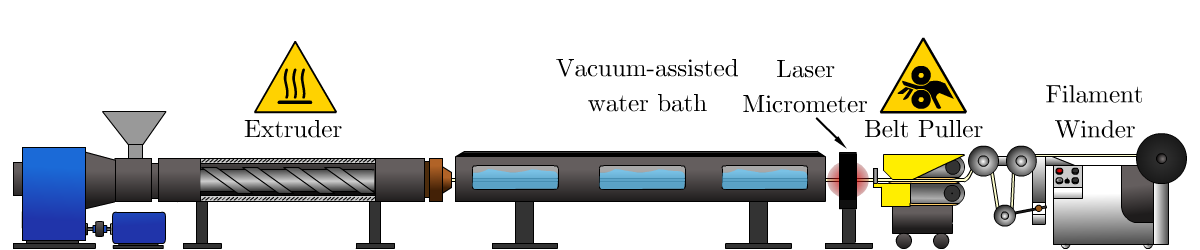
\includegraphics[width=\linewidth]{Extrusion_line}
	\caption{Extrusion line setup} \label{fig:extrLine}
\end{figure}
\pagebreak

\section{Sample Preparation}

As explained in Chapter \ref{ch:oocrit}, the OOC requires mechanical tests to obtain the multiple tensorial components of the mathematical function that describes part failure. Table \ref{tab:testsum} summarizes the tests required.
\begin{table} [h]
\centering
\caption{Summary of mechanical tests required}
\begin{tabular}{ c c } 
	\toprule
	\textbf{Mechanical Test} & \textbf{OOC parameters obtained} \\
	\midrule
	Tensile           &   $X_t$, $Y_t$\\
	Compressive       &   $X_c$, $Y_c$\\
	Torsion           &   $S$, $S_{45p}$ , $S_{45n}$\\
	Combined loading  &   $\mu^{1112}$ , $\mu^{2212}$\\
 	\bottomrule
\end{tabular}
\label{tab:testsum}
\end{table}

\subsection{Toolpath Planning}
\subsection{Printing Equipment}

\section{Mechanical Testing}
% Nomenclature introduced in this chapter:
\nomenclature[A]{ABS}{Acrylonitrile Butadiene Styrene}% 

% Symbols introduced in this chapter:
%\nomenclature[S]{$X_t$}{Tensile strength in the 1-1 direction \nomunit{$MPa$}}
\end{document}